% ===================== TracerTraj =====================
\subsection{TracerTraj (AgenTracer)}\label{ds:tracertraj}
\badgerow{\injected\ \naturalbadge\ \okbadge\ \lbl{agent + step}\ \lbl{MAS}\ \lbl{train + test}\ \lbl{MBPP+ / KodCode / MATH / GSM8K / GAIA / HotpotQA}}

\begin{identity}
Paper & \emph{AgenTracer: Who Is Inducing Failure in the LLM Agentic Systems?} --- Zhang, Wang, Chen, Zhou, Wang, Yan (OPPO, NUS, CUHK, NTU), ICLR 2026, arXiv:2509.03312 \cite{agentracer2026}\\
Links & \href{https://github.com/bingreeky/AgenTracer/releases/tag/data-v1.0.0}{GitHub \code{bingreeky/AgenTracer} release \code{data-v1.0.0}} \textperiodcentered\ \href{https://bingreeky.github.io/atracer/}{project page}; no Hugging Face release; AgenTracer-8B weights not released\\
License & none stated in the archive, README or repository\\
Status & downloaded in full (24 MB zip, 135 MB JSONL); 3,208 train + 790 test = 3,998 trajectories; \code{data/tracertraj/extracted/agentracer-data-v1.0.0/}. The release is larger than, and ``not identical'' to, the paper's TracerTraj-2.5K\\
\end{identity}

\paragraph{Description} TracerTraj is the \emph{training} resource behind AgenTracer-8B (Qwen3-8B tuned with GRPO and a step-Gaussian + agent-match reward), with held-out test splits per domain. Target = Who\&When's (responsible agent, decisive step). Labels are produced fully automatically, with no human review:
\begin{itemize}
\item \textbf{Collection}: six MAS---MetaGPT, AutoGen, Smolagents (hand-crafted), AgentPrune, AFlow, OWL-Workforce (automated)---on coding (MBPP+, KodCode, Blackjack), maths (MATH, GSM8K) and agentic (GAIA, HotpotQA) tasks.
\item \textbf{Counterfactual replay} of natural failures: a DeepSeek-R1 analyser with access to the ground truth proposes a minimal fix at each step and the run is re-simulated; the earliest fix that yields success marks the decisive step (``Diagnosis Error'').
\item \textbf{Programmatic fault injection} into successful runs: a perturbation operator corrupts one sampled action; if the run then fails, that step is the label by construction (``Injection Error'').
\end{itemize}
Paper composition (TracerTraj-2.5K): 1,288 coding / 630 math / 558 agentic annotated, 9:1 train/test. The released v1.0.0 has 1,268 coding / 630 math / 2,100 agentic rows, curated from a different data version, with 690 e-mail and 88 credential strings redacted to placeholders. In the agentic domain 1,822 rows are injected and 278 diagnosed; coding and math carry no \code{error\_source}, so the injected/natural split is not recoverable there. No failure taxonomy; \code{mistake\_reason} and \code{ground\_truth} exist for coding/math only.

\paragraph{Metrics and baselines} All-at-once attribution, output \code{<agentID> | <stepID>}; agent- and step-level accuracy, each with (w/\,G) and without (w/o\,G) the task ground truth. TracerTraj test splits, w/\,G, agent\,/\,step accuracy in \% (paper):

\begin{center}\small
\begin{tabular}{@{}lccc@{}}\toprule
Model & Code & Math & Agentic\\\midrule
Qwen3-8B & 45.4 / 2.4 & 31.7 / 9.5 & 27.9 / 13.5\\
GPT-4.1 & 59.8 / 12.6 & 39.6 / 35.8 & 43.6 / 25.0\\
DeepSeek-R1 & 11.8 / 10.2 & 42.7 / 29.5 & 45.1 / 27.1\\
Gemini-2.5-Pro & 70.1 / 11.0 & 58.8 / 32.2 & 37.2 / 18.6\\
Claude-Sonnet-4 & 66.0 / 15.5 & 46.0 / 38.1 & \textbf{55.2} / 30.3\\
AgenTracer-8B & \textbf{73.0} / \textbf{18.9} & \textbf{59.3} / \textbf{57.6} & 53.3 / \textbf{36.2}\\\bottomrule
\end{tabular}
\end{center}
On Who\&When (w/\,G) AgenTracer-8B reaches 69.1\,/\,20.7 (Hand-Crafted) and 69.6\,/\,42.9 (Alg.-Generated) versus 56.9\,/\,17.2 and 57.9\,/\,40.7 for Claude-Sonnet-4. Step accuracy on code is low for every model.

\paragraph{Schema} \code{\{agentic,coding,math\}/\{train,test\}.jsonl} plus \code{MANIFEST.json} (row counts, SHA-256, redaction counts). Row fields: \code{question\_ID} (not unique: 118 math ids recur as injected variants, 21 ids occur in both splits), \code{question}, \code{history} (list of \{\code{step}, \code{content}, \code{role}, \code{name}\}), \code{mistake\_agent}, \code{mistake\_step} (stored as a \emph{string}; \code{step} is 1-based in agentic, 0-based in coding/math), \code{mistake\_reason} and \code{ground\_truth} (coding/math), \code{error\_source} (agentic). Agentic rows have no \code{name}: every step is the generic \code{assistant}. Coding roles are MetaGPT's Team Leader / Product Manager / Architect / Engineer / Data Analyst; math ``agents'' are AFlow operators (\code{Custom}, \code{reasoning expert}, \ldots).

\paragraph{Statistics} computed from the released archive (train + test pooled).\par\nobreak\vspace{1pt}
\noindent\begin{minipage}[t]{0.55\linewidth}\vspace{0pt}\small
\fitbox{\begin{tabular}{@{}lrrrr@{}}\toprule
 & All & Agentic & Coding & Math\\\midrule
trajectories: train + test & 3208 + 790 & 1500 + 600 & 1141 + 127 & 567 + 63\\
steps: mean / median & 12.5 / 10 & 9.4 / 7 & 20.9 / 14 & 6.3 / 7\\
steps: min -- max & 1 -- 304 & 4 -- 42 & 1 -- 304 & 3 -- 11\\
named agents / traj.: mean & 1.7 & 1 & 2.3 & 2.7\\
relative error position: mean & 0.52 & 0.55 & 0.46 & 0.54\\
error at the last step & 470 & -- & -- & --\\
characters / traj.: mean & 31\,k & 36\,k & 35.5\,k & 8.5\,k\\
injected / diagnosed labels & -- & 1822 / 278 & n/a & n/a\\\bottomrule
\end{tabular}}

\smallskip Blamed agent: agentic \code{assistant} 2,100 (100\%); coding Engineer 935, Product Manager 155, Team Leader 125, Architect 46; math \code{Custom} 400, \code{reasoning expert} 171, \code{BestMAS\_GSM8K} 55. The sender of the labelled step equals \code{mistake\_agent} in 100\% of rows. 1,212 rows place the error in the last 30\% of the trajectory; $\approx$8\,k tokens per trajectory on average.
\end{minipage}\hfill
\begin{minipage}[t]{0.43\linewidth}\vspace{0pt}
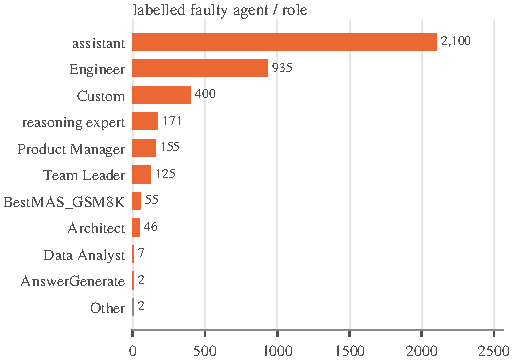
\includegraphics[width=\linewidth]{4_injected/tracertraj/figures/agent.pdf}
\end{minipage}

\paragraph{Example trajectory} \code{coding/test} record \code{Filter\_5086\_I} (MetaGPT team, 8 steps, 2 roles, 16.7\,k characters). The Team Leader delegates a trivial \code{find\_duplicates} function to the Product Manager, who writes a requirements document into \code{solution.py} instead of code (step 6); no implementation is ever produced.
% auto-generated by scripts/render_traj.py -- do not edit
\trajtask{Filter\_5086\_I}{Please solve the programming task below in Python.\par Given a non-empty list of integers,\allowbreak{} write a Python function that returns a new list containing the elements that appear twice in the original list. The function should handle duplicate entries and empty lists.\par Note that the function declaration is def find\_duplicates(nums):\allowbreak{}. }
\begin{trajstep}{0}{Team Leader}{agA}
Team Leader thinking:\allowbreak{}\newline \# Past Experience\newline <experience>\par \# Tool State\par \# Current Plan\newline [GOAL] [Message] from User to Mike:\allowbreak{} Please solve the programming task below in Python.\par Given a non-empty list of integers,\allowbreak{} write a Python function that returns a new list containing the elements that appear twice in the original list. The function should handle duplicate entries and empty lists.\par Note that the function declaration is def find\_duplicates(nums):\allowbreak{}. I wish you finish the task with a multi-agent cooperationThe file name of your solution must be 'solution.py'\newline No Plan\par \# Current Task\par \# Response Language\newline you must respond in English.\par Pay close\newline [...] (1,\allowbreak{}368 chars omitted) [...]\newline d adhere to the following format.\newline ```json\newline [\newline \{\newline "command\_name":\allowbreak{} "ClassName.method\_name" or "function\_name",\allowbreak{}\newline "args":\allowbreak{} \{"arg\_name":\allowbreak{} arg\_value,\allowbreak{} ...\}\newline \},\allowbreak{}\newline ...\newline ]\newline ```\newline Notice:\allowbreak{} your output JSON data section must start with **```json [**
\end{trajstep}
\begin{trajstep}{1}{Team Leader}{agA}
Team Leader thinking:\allowbreak{} To address the user's request,\allowbreak{} I will create a plan that involves multiple team members. The task requires writing a Python function to find duplicates in a list,\allowbreak{} which can be handled efficiently by the Engineer. However,\allowbreak{} since the user requested multi-agent cooperation,\allowbreak{} I will also involve the Product Manager to create a Product Requirement Document (PRD) for clarity and documentation purposes.\par Here's the plan:\allowbreak{}\newline 1. Alice (Product Manager) will create a PRD based on the user's requirement.\newline 2. Alex (Engineer) will implement the function `find\_duplicates(nums)` in a file named `solution.py`.\par I will start by assigning th\newline [...] (1,\allowbreak{}215 chars omitted) [...]\newline nd\_name":\allowbreak{} "RoleZero.reply\_to\_human",\allowbreak{}\newline "args":\allowbreak{} \{\newline "content":\allowbreak{} "I have assigned the task to Alice to create the PRD. Once it's completed,\allowbreak{} Alex will implement the function."\newline \}\newline \},\allowbreak{}\newline \{\newline "command\_name":\allowbreak{} "end"\newline \}\newline ]\newline ```
\end{trajstep}
\begin{trajstep}{2}{Team Leader}{agA}
Team Leader sends to Alice:\allowbreak{} Create a Product Requirement Document (PRD) for the task:\allowbreak{} Given a non-empty list of integers,\allowbreak{} write a Python function that returns a new list containing the elements that appear twice in the original list. The function should handle duplicate entries and empty lists. The function declaration is def find\_duplicates(nums):\allowbreak{}. The solution file name must be 'solution.py'.
\end{trajstep}
\begin{trajstep}{3}{Product Manager}{agB}
Product Manager thinking:\allowbreak{}\newline \# Past Experience\newline <experience>\par \# Tool State\par \# Current Plan\newline [GOAL] [Message] from Mike to Alice:\allowbreak{} Create a Product Requirement Document (PRD) for the task:\allowbreak{} Given a non-empty list of integers,\allowbreak{} write a Python function that returns a new list containing the elements that appear twice in the original list. The function should handle duplicate entries and empty lists. The function declaration is def find\_duplicates(nums):\allowbreak{}. The solution file name must be 'solution.py'.\newline No Plan\par \# Current Task\par \# Response Language\newline you must respond in English.\par Pay close attention to the Example provided,\allowbreak{} you can reuse the example for\newline [...] (1,\allowbreak{}303 chars omitted) [...]\newline d adhere to the following format.\newline ```json\newline [\newline \{\newline "command\_name":\allowbreak{} "ClassName.method\_name" or "function\_name",\allowbreak{}\newline "args":\allowbreak{} \{"arg\_name":\allowbreak{} arg\_value,\allowbreak{} ...\}\newline \},\allowbreak{}\newline ...\newline ]\newline ```\newline Notice:\allowbreak{} your output JSON data section must start with **```json [**
\end{trajstep}
\begin{trajstep}{4}{Product Manager}{agB}
Product Manager thinking:\allowbreak{} To create a Product Requirement Document (PRD) for the task of writing a Python function that identifies duplicate integers in a list,\allowbreak{} I will first outline the necessary sections of the PRD. This will include the language and project info,\allowbreak{} product definition,\allowbreak{} technical specifications,\allowbreak{} and any open questions.\par I will start by creating a new file named 'solution.py' to hold the function implementation. After that,\allowbreak{} I will insert the PRD content into the file.\par Here's the plan:\allowbreak{}\newline 1. Create the file 'solution.py'.\newline 2. Insert the PRD content into the file.\par Let's proceed with creating the file first.\par ```json\newline [\newline \{\newline "command\_name":\allowbreak{} "Editor.create\_file",\allowbreak{}\newline "args":\allowbreak{} \{"filename":\allowbreak{} "solution.py"\}\newline \}\newline ]\newline ```
\end{trajstep}
\begin{trajstep}{5}{Product Manager}{agB}
Product Manager thinking:\allowbreak{}\newline \# Past Experience\newline <experience>\par \# Tool State\par \# Current Plan\newline [GOAL] [Message] from Mike to Alice:\allowbreak{} Create a Product Requirement Document (PRD) for the task:\allowbreak{} Given a non-empty list of integers,\allowbreak{} write a Python function that returns a new list containing the elements that appear twice in the original list. The function should handle duplicate entries and empty lists. The function declaration is def find\_duplicates(nums):\allowbreak{}. The solution file name must be 'solution.py'.\newline No Plan\par \# Current Task\par \# Response Language\newline you must respond in English.\par Pay close attention to the Example provided,\allowbreak{} you can reuse the example for\newline [...] (1,\allowbreak{}303 chars omitted) [...]\newline d adhere to the following format.\newline ```json\newline [\newline \{\newline "command\_name":\allowbreak{} "ClassName.method\_name" or "function\_name",\allowbreak{}\newline "args":\allowbreak{} \{"arg\_name":\allowbreak{} arg\_value,\allowbreak{} ...\}\newline \},\allowbreak{}\newline ...\newline ]\newline ```\newline Notice:\allowbreak{} your output JSON data section must start with **```json [**
\end{trajstep}
\begin{faultystep}{6}{Product Manager}{agB}
Product Manager thinking:\allowbreak{} I will now insert the PRD content into the 'solution.py' file. The PRD will include the language and project info,\allowbreak{} product definition,\allowbreak{} technical specifications,\allowbreak{} and open questions. This will provide a comprehensive overview of the task requirements.\par Here's the content I will insert:\allowbreak{}\par ```markdown\newline \# Product Requirement Document (PRD)\par \#\# 1. Language \& Project Info\newline - **Language**:\allowbreak{} Python\newline - **Project Name**:\allowbreak{} find\_duplicates\_function\par \#\# 2. Product Definition\newline \#\#\# Product Goals\newline 1. Identify and return elements that appear twice in a list of integers.\newline 2. Handle duplicate entries effectively.\newline 3. Ensure the function can man\newline [...] (2,\allowbreak{}605 chars omitted) [...]\newline for performance.\textbackslash{}n\textbackslash{}n\#\#\# UI Design Draft\textbackslash{}n- Input:\allowbreak{} List of integers\textbackslash{}n- Output:\allowbreak{} List of duplicates\textbackslash{}n\textbackslash{}n\#\#\# Open Questions\textbackslash{}n- What should the function return if the input list is empty?\allowbreak{}\textbackslash{}n- Are there any performance benchmarks we should consider?\allowbreak{}\textbackslash{}n"\}\newline ]\newline ```
\end{faultystep}
\begin{trajstep}{7}{Product Manager}{agB}
Product Manager thinking:\allowbreak{}\newline \# Past Experience\newline <experience>\par \# Tool State\par \# Current Plan\newline [GOAL] [Message] from Mike to Alice:\allowbreak{} Create a Product Requirement Document (PRD) for the task:\allowbreak{} Given a non-empty list of integers,\allowbreak{} write a Python function that returns a new list containing the elements that appear twice in the original list. The function should handle duplicate entries and empty lists. The function declaration is def find\_duplicates(nums):\allowbreak{}. The solution file name must be 'solution.py'.\newline No Plan\par \# Current Task\par \# Response Language\newline you must respond in English.\par Pay close attention to the Example provided,\allowbreak{} you can reuse the example for\newline [...] (1,\allowbreak{}303 chars omitted) [...]\newline d adhere to the following format.\newline ```json\newline [\newline \{\newline "command\_name":\allowbreak{} "ClassName.method\_name" or "function\_name",\allowbreak{}\newline "args":\allowbreak{} \{"arg\_name":\allowbreak{} arg\_value,\allowbreak{} ...\}\newline \},\allowbreak{}\newline ...\newline ]\newline ```\newline Notice:\allowbreak{} your output JSON data section must start with **```json [**
\end{trajstep}
\trajannotation{Product Manager}{6}{—}{The Product Manager created a PRD and inserted it into the solution.py file,\allowbreak{} but did not implement the actual function 'find\_duplicates(nums)'. The task requires a functional implementation,\allowbreak{} not just documentation.}{def find\_duplicates(nums):\allowbreak{}\newline """\newline Given a list of integers,\allowbreak{} return a new list containing the elements that appear twice in the original list.\par Arguments:\allowbreak{}\newline nums -- list of integers\par Returns:\allowbreak{}\newline [...] (63 chars omitted) [...]\newline count =\allowbreak{} Counter(nums)\newline return [num for num,\allowbreak{} cnt in count.items() if cnt =\allowbreak{}=\allowbreak{} 2]}{Product Manager thinking:\allowbreak{}\newline \# Past Experience\newline <experience>\par \# Tool State\par \# Current Plan\newline [GOAL] [Message] from Mike to Alice:\allowbreak{} Create a Product Requirement Document (PRD) for the task:\allowbreak{} Giv\newline [...] (1,\allowbreak{}943 chars omitted) [...]\newline ```\newline Notice:\allowbreak{} your output JSON data section must start with **```json [**}{\textbf{domain}: coding; \textbf{split}: test; \textbf{file}: coding/\allowbreak{}test.jsonl; \textbf{step\_indexing}: field history[].step,\allowbreak{} first step =\allowbreak{} 0; \textbf{mistake\_step\_raw\_type}: str}


\paragraph{Notes} (i) Labels are synthetic (counterfactual replay or injection, both driven by DeepSeek-R1) and unvalidated by humans; the paper reports no agreement figures, and the release differs from the paper's TracerTraj-2.5K. (ii) The agentic domain (53\% of rows) labels every step as \code{assistant}, so agent-level accuracy is trivially 100\% there and only the step matters; the paper's agentic agent-accuracy numbers (27--55\%) are therefore not reproducible from this release. (iii) Short but heavy: median 10 steps, yet 31\,k characters per trajectory because steps embed large tool/web outputs (partly in Chinese); coding runs reach 304 steps. (iv) Error position skews late: 470 rows put the decisive error at the last step. (v) Indexing inconsistencies (string \code{mistake\_step}, 1- vs 0-based \code{step}) and task-level leakage between train and test (21 shared \code{question\_ID}s). (vi) Frameworks and benchmarks overlap with MAST and AEGIS (same first author as AEGIS), but all runs are the authors' own; Who\&When is the external test set.
